% Software layers behind the SPI bus diagram (spi-bus.tex): the host's device.py sends text commands to the
% ESP32 serial CLI (isingmachine.ino), which calls machine/couplers (write weights, decoder addresses 0-6) or
% machine/oscillators (read spins, address 7). Those use the drivers mcp4351 (SPI mode 0) and hcs165
% (SPI mode 2), which sequence the shared bus (bus.cpp): ADDR, CS1, SH/LD and SCLK/MOSI/MISO.
% Build: lualatex software-overview.tex && pdftoppm -png -r 300 -singlefile software-overview.pdf software-overview
\documentclass[border=8pt]{standalone}
\usepackage{tikz}
\usetikzlibrary{arrows.meta}
\usepackage{fontspec}
\setmainfont{TeX Gyre Heros}

\begin{document}
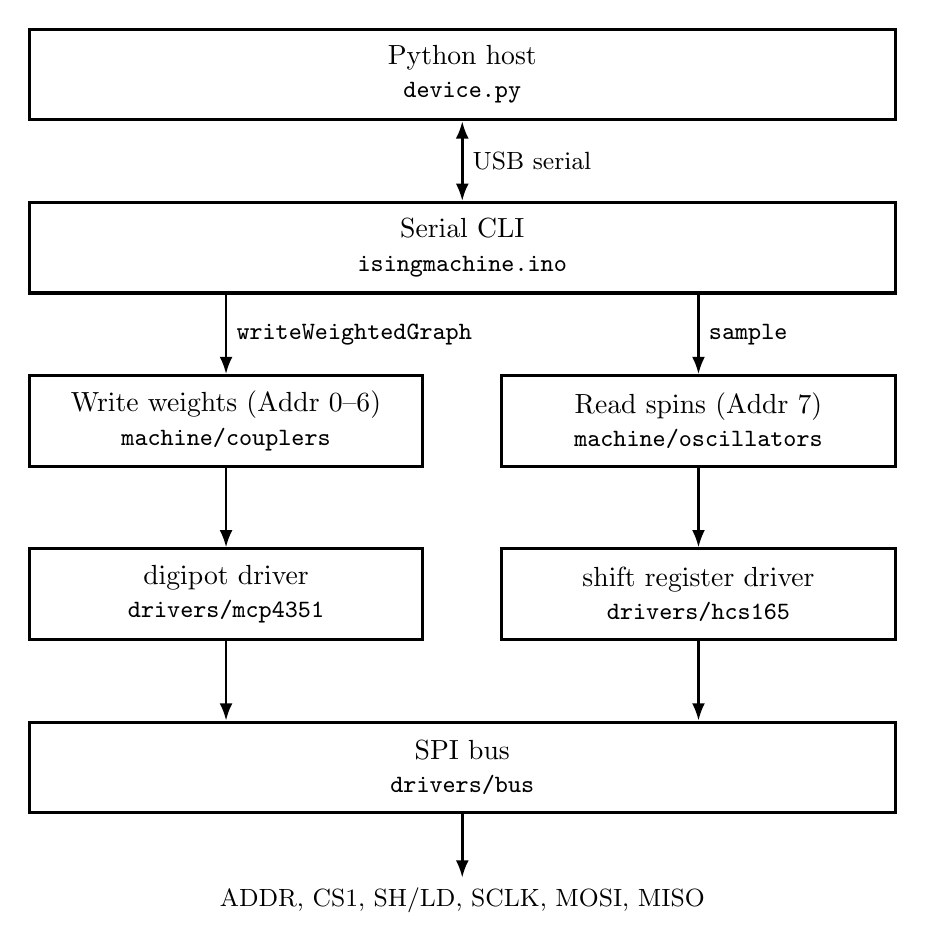
\begin{tikzpicture}[
    font=\normalsize, line width=0.9pt, >={Latex[length=2.2mm]},
    box/.style={draw, line width=1.1pt, minimum height=1.15cm, align=center},
    wide/.style={box, minimum width=11cm},
    col/.style={box, minimum width=5cm},
    lbl/.style={font=\small, align=center},
    f/.style={font=\small\ttfamily},
  ]
  \node[wide] (dev) at (3,0) {Python host\\{\small\ttfamily device.py}};
  \node[wide] (cli) at (3,-2.2) {Serial CLI\\{\small\ttfamily isingmachine.ino}};
  \draw[<->] (dev) -- node[lbl, right] {USB serial} (cli);

  \node[col] (cpl) at (0,-4.4) {Write weights (Addr 0--6)\\{\small\ttfamily machine/couplers}};
  \node[col] (osc) at (6,-4.4) {Read spins (Addr 7)\\{\small\ttfamily machine/oscillators}};
  \draw[->] (cpl |- cli.south) -- node[f, right] {writeWeightedGraph} (cpl);
  \draw[->] (osc |- cli.south) -- node[f, right] {sample} (osc);

  \node[col] (mcp) at (0,-6.6) {digipot driver\\{\small\ttfamily drivers/mcp4351}};
  \node[col] (hcs) at (6,-6.6) {shift register driver\\{\small\ttfamily drivers/hcs165}};
  \draw[->] (cpl) -- (mcp);
  \draw[->] (osc) -- (hcs);

  \node[wide] (bus) at (3,-8.8) {SPI bus\\{\small\ttfamily drivers/bus}};
  \draw[->] (mcp) -- (mcp |- bus.north);
  \draw[->] (hcs) -- (hcs |- bus.north);

  \draw[->] (bus) -- ++(0,-1.4) node[below, lbl] {ADDR, CS1, SH/LD, SCLK, MOSI, MISO};
\end{tikzpicture}
\end{document}
